\documentclass[11pt, a4paper, twoside]{article}
% questi due pacchetti servono per indicare la codifica della tastiera usata e i caratteri che vogliamo usare.
% a noi non servono molto, ma metti che compiliamo con un computer russo?
\usepackage[T1]{fontenc}
\usepackage[utf8]{inputenc}
%non capisco il perché della metà dei pacchetti kek
\usepackage{blindtext}
\usepackage{geometry}
\usepackage{setspace}
\usepackage{titlesec}
\usepackage{indentfirst}
\usepackage{graphicx}
\usepackage[italian]{babel}
\usepackage{catchfile} % used in \getenv command
\usepackage{multicol}
\usepackage{amsmath}
\usepackage{subcaption}
\usepackage[hang, flushmargin, multiple, bottom]{footmisc}
\usepackage{float}
\usepackage{array}
\usepackage{booktabs}
\usepackage{url}
\usepackage{csvsimple}


\titlespacing*{\section}{0px}{3mm}{1mm}         %what purpouse?
\titlespacing*{\subsection}{0px}{3mm}{1mm}      %what purpouse?
\geometry{
  left=2cm,
  right=2cm,
  top=2cm,
  bottom=2cm
}
\setlength{\parindent}{10mm}
\graphicspath{ {./assets}, {../../assets} }

% Allow use of command \getenv{VARNAME}.
% Taken from: https://tex.stackexchange.com/questions/62010/can-i-access-system-environment-variables-from-latex-for-instance-home
\newcommand{\getenv}[2][]{
  \CatchFileEdef{\temp}{"|kpsewhich --var-value #2"}{\endlinechar=-1}%
  \if\relax\detokenize{#1}\relax\temp\else\let#1\temp\fi}

% Roman numerals
\newcommand{\rom}[1]{\uppercase\expandafter{\romannumeral #1\relax}}


% authors, date and title---------------------------------------------------------------
\author{Giuseppe Sguera \\ \getenv{MAT1} \and Matteo Bonacini \\ \getenv{MAT2}}
\date{\today}
\title{Misura della caratteristica I-V di due diodi a semiconduttore}
%---------------------------------------------------------------------------------------
\begin{document}

%\twocolumn[
%  \begin{@twocolumnfalse}
    %\begin{center}
{
	{\Large
		{\textsc{Alma Mater Studiorum $\cdot$ Università di Bologna}}
	}
}
\rule[0.1cm]{18cm}{0.1mm}
\rule[0.5cm]{18cm}{0.6mm}
{\small
	{\bf SCUOLA DI SCIENZE\\
		Corso di Laurea in Fisica
	}
}
{\let\newpage\relax\maketitle}
\end{center}


    \maketitle

    \begin{abstract}\label{sec:abstract}
      In questa prova abbiamo misurato l'andamento I-V di due diodi a semiconduttore diversi (Silicio e Germanio), per poi svolgere un \emph{fit}
      sui dati raccolti e ricavare i parametri $I_0$ e $\eta V_T$. La prova è servita anche come addestramento all'utilizzo
      un oscilloscopio analogico. I risultati dei \emph{fit} sono compatibili con il range di valori atteso.
    \end{abstract}
% \end{@twocolumnfalse}
%]

\section{Introduzione}\label{sec:scopo}
  La caratteristica I-V di un diodo al silicio contiene tutte le informazioni necessarie per descriverne il comportamento.
  Per correnti piccole, l'andamento previsto dalla teoria è riassunto dall'Equazione di Shockley \eqref{eq:shockley}:
  \begin{equation}
    I(V_d) = I_0 \left(
      e^{
        \frac {V_d} {\eta V_T}
      } - 1
    \right)
    \label{eq:shockley}
  \end{equation}
  dove $V_d$ è la tensione applicata ai capi del diodo, $\eta$ è il \emph{fattore di idealità}, $V_T$ è un parametro dipendente dalla
  temperatura e $I_0$ è la corrente inversa. Per ulteriori informazioni, si rimanda a \cite{halkias2001integrated}.
  Aumentando la corrente oltre una certa soglia, l'andamento diventa sub-esponenziale e non rispetta più l'equazione \eqref{eq:shockley}.

  Lo scopo principale di questa prova è di misurare l'andamento I-V di due diodi a semiconduttore diversi (vedi sezione \ref{subsec:materiali}), per poi svolgere un
  \emph{fit} del loro andamento nel limite di validità dell'equazione \eqref{eq:shockley}. Dal fit verranno estratti i parametri $I_0$ e $\eta V_T$.
  In secondo luogo, questa prova serve anche come addestramento per imparare ad usare un oscilloscopio analogico, in funzione delle successive
  prove di laboratorio.


\section{Apparato sperimentale}\label{sec:apparato-sperimentale}
  \subsection{Schema del circuito}\label{subsec:schema-circuito}
    \begin{figure}%[H]
      \centering
      \begin{subfigure}[t]{.47\textwidth}
        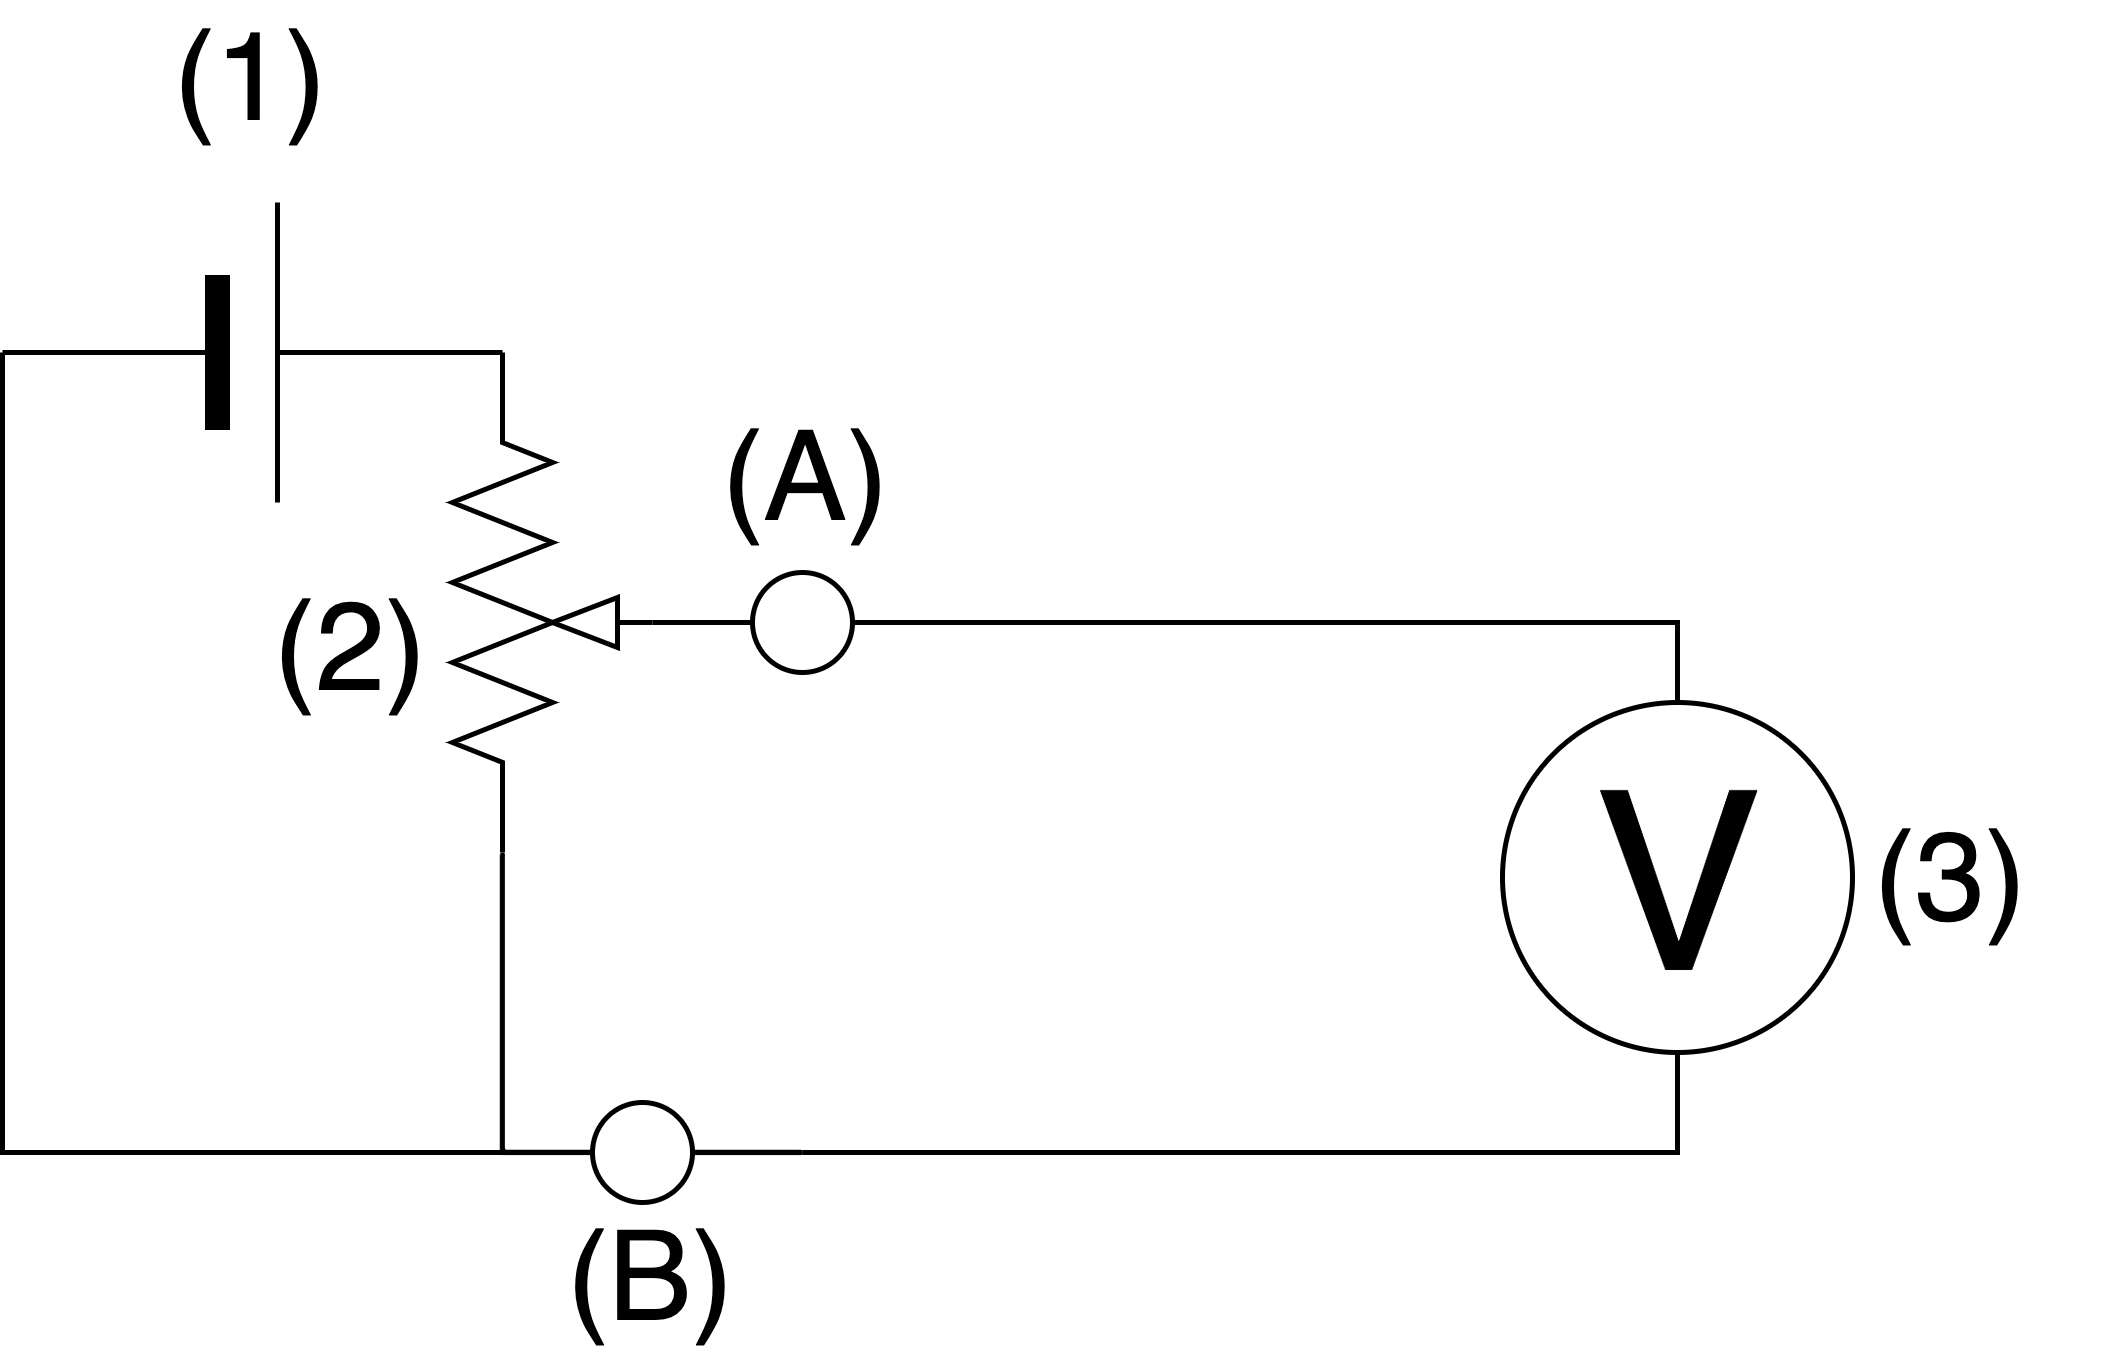
\includegraphics[width=8.75cm]{./assets/1/circuito-calibrazione.png}
        \caption{
          \emph{
            Schema del circuito usato per la calibrazione. Il generatore (1) è collegato al potenziometro (2).
            Il multimetro (3) misura il potenziale tra terra e il pin intermedio del potenziometro.
            L'oscilloscopio (non riportato) è collegato a terra e al punto (A).
          }
        }
        \label{fig:circuito-calibrazione}
      \end{subfigure}
      %
      \hspace{5mm}
      %
      \begin{subfigure}[t]{.47\textwidth}
        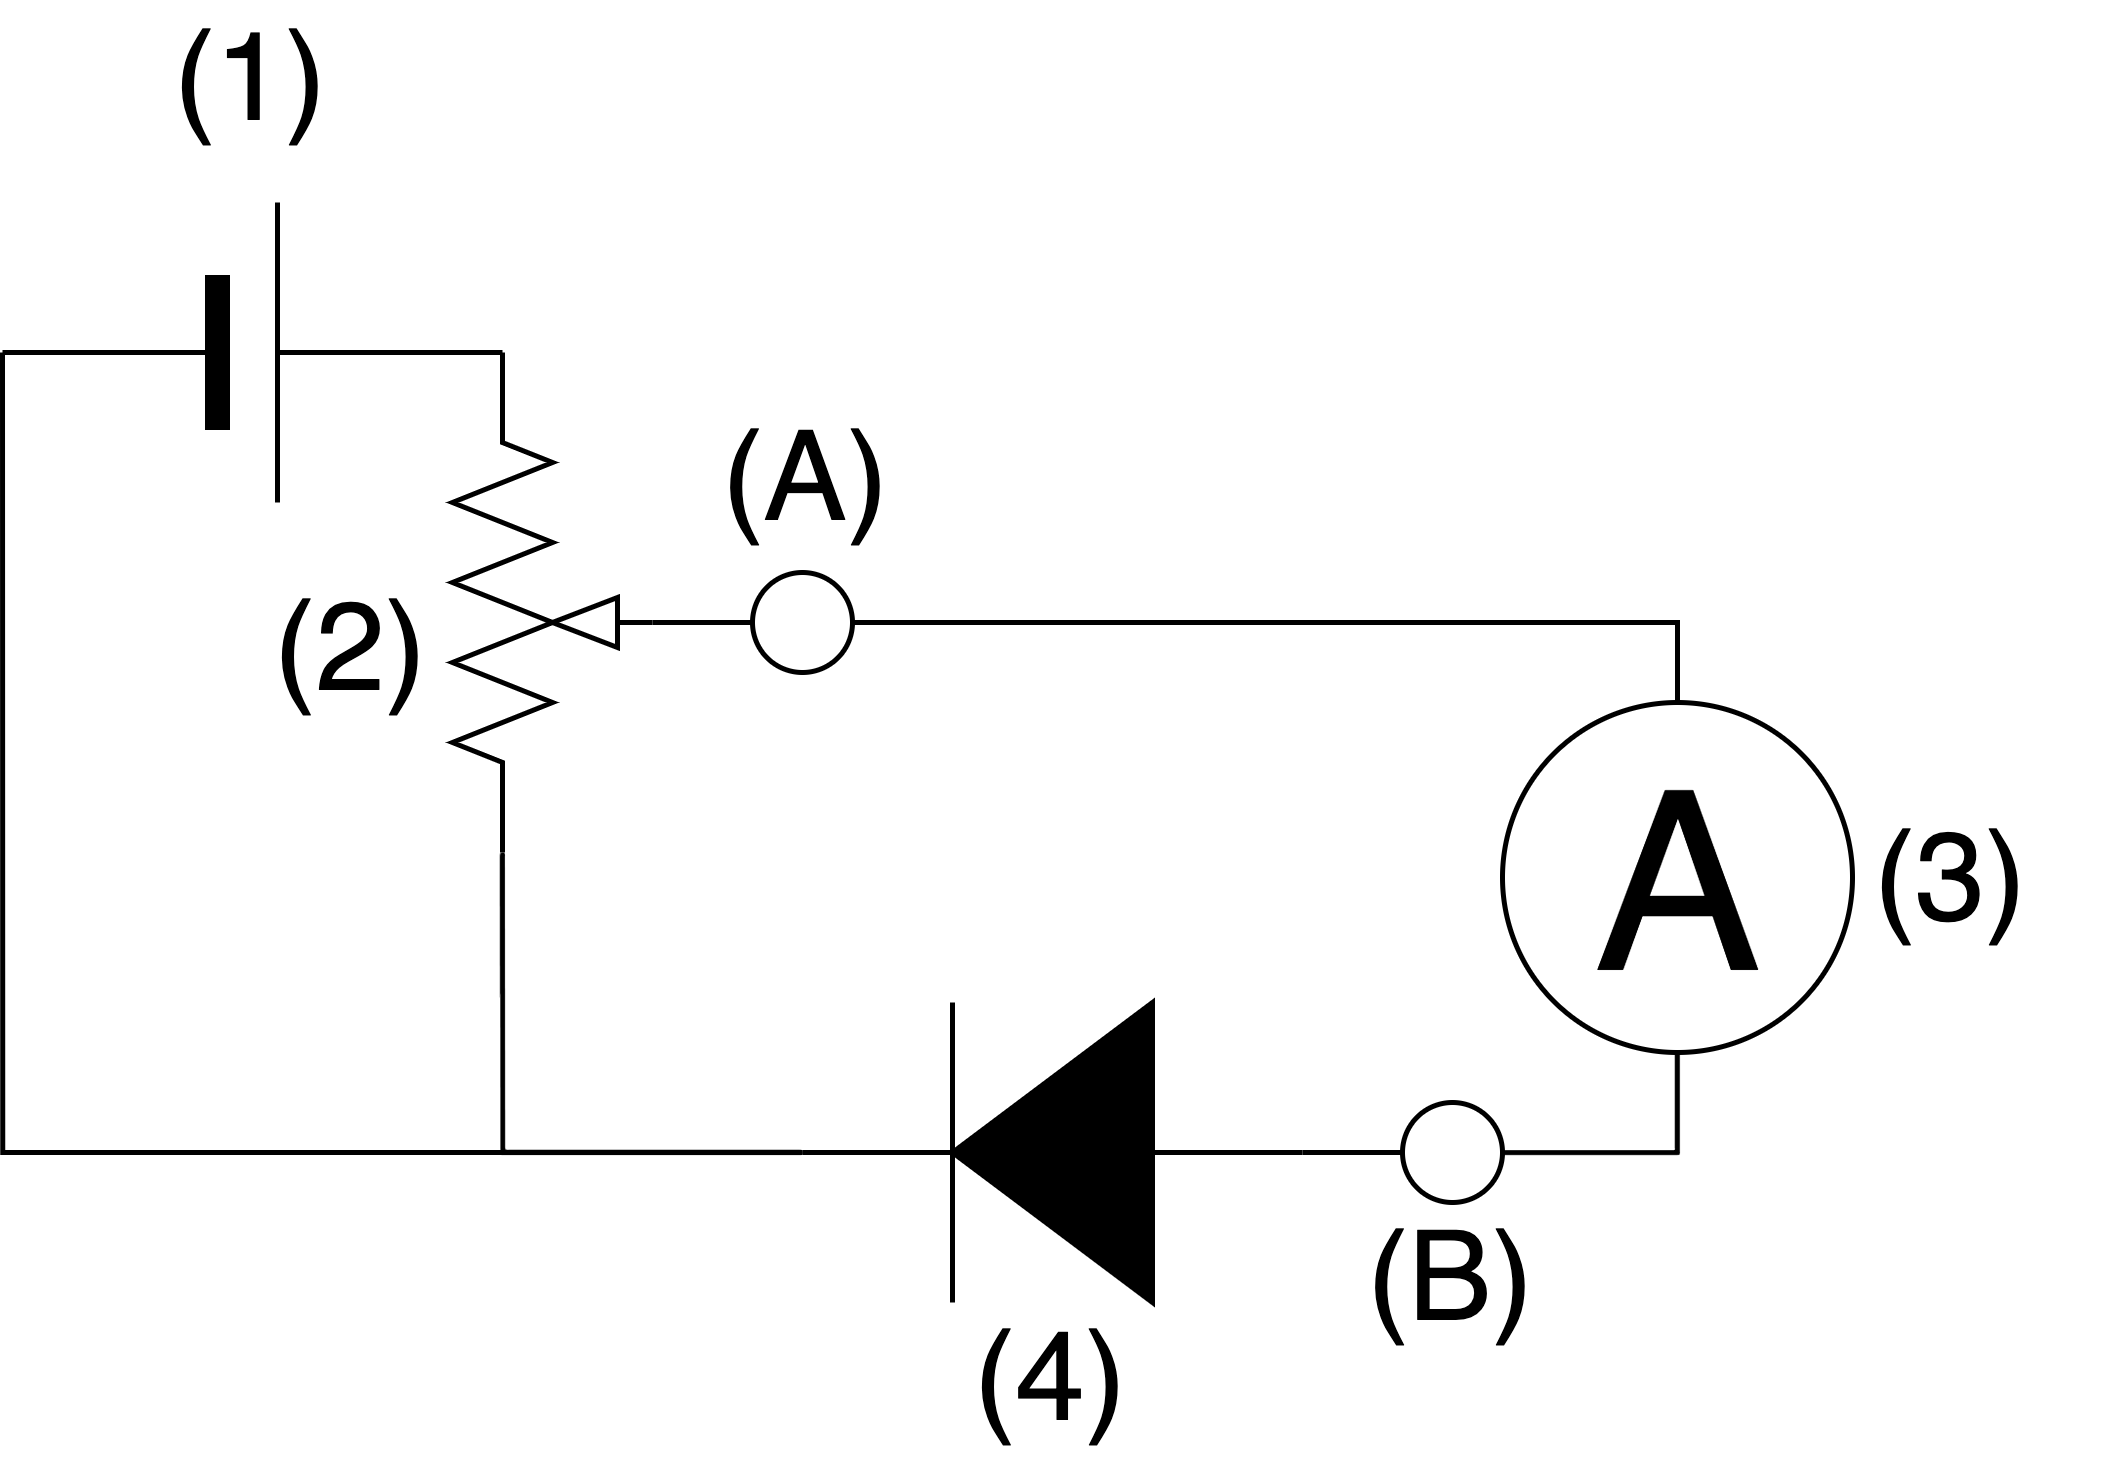
\includegraphics[width=8.75cm]{./assets/1/circuito.png}
        \caption{
          \emph{
            Schema del circuito usato per l'esperimento. Il generatore (1) è collegato al potenziometro (2).
            Il multimetro (3) misura la corrente che scorre nel diodo (4). L'oscilloscopio (non riportato) è
            collegato a terra e al punto (B).
          }
        }
        \label{fig:circuito-prova}
      \end{subfigure}
      \caption{\emph{Schemi circuitali.}}
      \label{fig:circuiti}
    \end{figure}

    Il circuito che abbiamo realizzato è schematizzato in figura \ref{fig:circuiti}, in due configurazioni diverse. In figura \ref{fig:circuito-calibrazione}
    è riportata la configurazione usata per controllare la calibrazione degli strimenti; in figura \ref{fig:circuito-prova}
    è riportata quella usata durante l'esperimento. Il circuito per l'esperimento è strutturato come segue:
    \begin{enumerate}
      \item%
        Un generatore di tensione costante di $5V$ è collegato ai \emph{pin} fissi di un potenziometro.
      \item%
        Il \emph{pin} variabile del potenziometro è collegato in serie a un multimetro e a un diodo.
      \item%
        Un osciolloscopio è collegato a terra e al punto $(B)$ del circuito.
    \end{enumerate}
    Per ottenere il circuito di calibrazione, è sufficiente cortocircuitare il diodo e collegare l'oscilloscopio al punto $(A)$.

  \subsection{Materiale e strumenti usati}\label{subsec:materiali}
    Segue una lista del materiale e degli strumenti usati durante la prova:
      \begin{itemize}
        \item%
          Oscilloscopio analogico, modello: \emph{GW Instek GOS-652}.
        \item%
          Multimetro digitale, modello: \emph{ISO-TECH IDM 105}.
        \item%
          Generatore di tensione, modello: \emph{Aim-TTi EB2025T}.
        \item%
          Sonda per oscilloscopio.
        \item%
          Connettori vari (connettori a banana, cavi per la scheda millefori).
        \item%
          Diodo al Silicio, modello: \emph{1N4148}.
        \item%
          Diodo al Germanio, modello: \emph{OA47}.
        \item
          Potenziometro da 1k$\Omega$.
      \end{itemize}
    Le incertezze degli strumenti utilizzati sono riportate in appendice \ref{sec:incertezze-strumentali}.
    Abbiamo considerato trascurabili le incertezze delle misure fatte con il multimetro, rispetto a quelle fatte con l'oscilloscopio.

\section{Risultati}\label{sec:risultati}
  Non è stato necessario aggiungere una correzione per la mancata calibrazione degli strumenti, visto che le misure di
  tensione sono compatibili entro il $3\%$.
  I valori numerici dei dati raccolti sono riportati in appendice \ref{sec:valori-misure}.
  I risultati dei \emph{fit} sono riportati in tabella \ref{tab:risultati-fit}.
  In figura \ref{fig:caratteristiche-iv} sono riportati i grafici delle caratteristiche I-V dei due diodi.
  \begin{table}[H]
    \centering
    \begin{tabular}[t]{ccc}
      \toprule
      Diodo& Parametro &Valore ottenuto\\
      \midrule
      Si & $I_0$ &  $(2.3 \pm 1.8)\:nA$ \\
      Si & $\eta V_T$ &  $(48 \pm 4)\:mV$ \\
      Ge & $I_0$ &  $(1.6 \pm 0.4)\:\mu A$ \\
      Ge & $\eta V_T$ &  $(35 \pm 3)\:mV$ \\
      \bottomrule
      \end{tabular}
    \caption{
      Risultati dei \emph{fit} dei dati raccolti.
    }
    \label{tab:risultati-fit}
  \end{table}
  \begin{figure}%[H]
    \centering
    \begin{subfigure}[t]{.47\textwidth}
      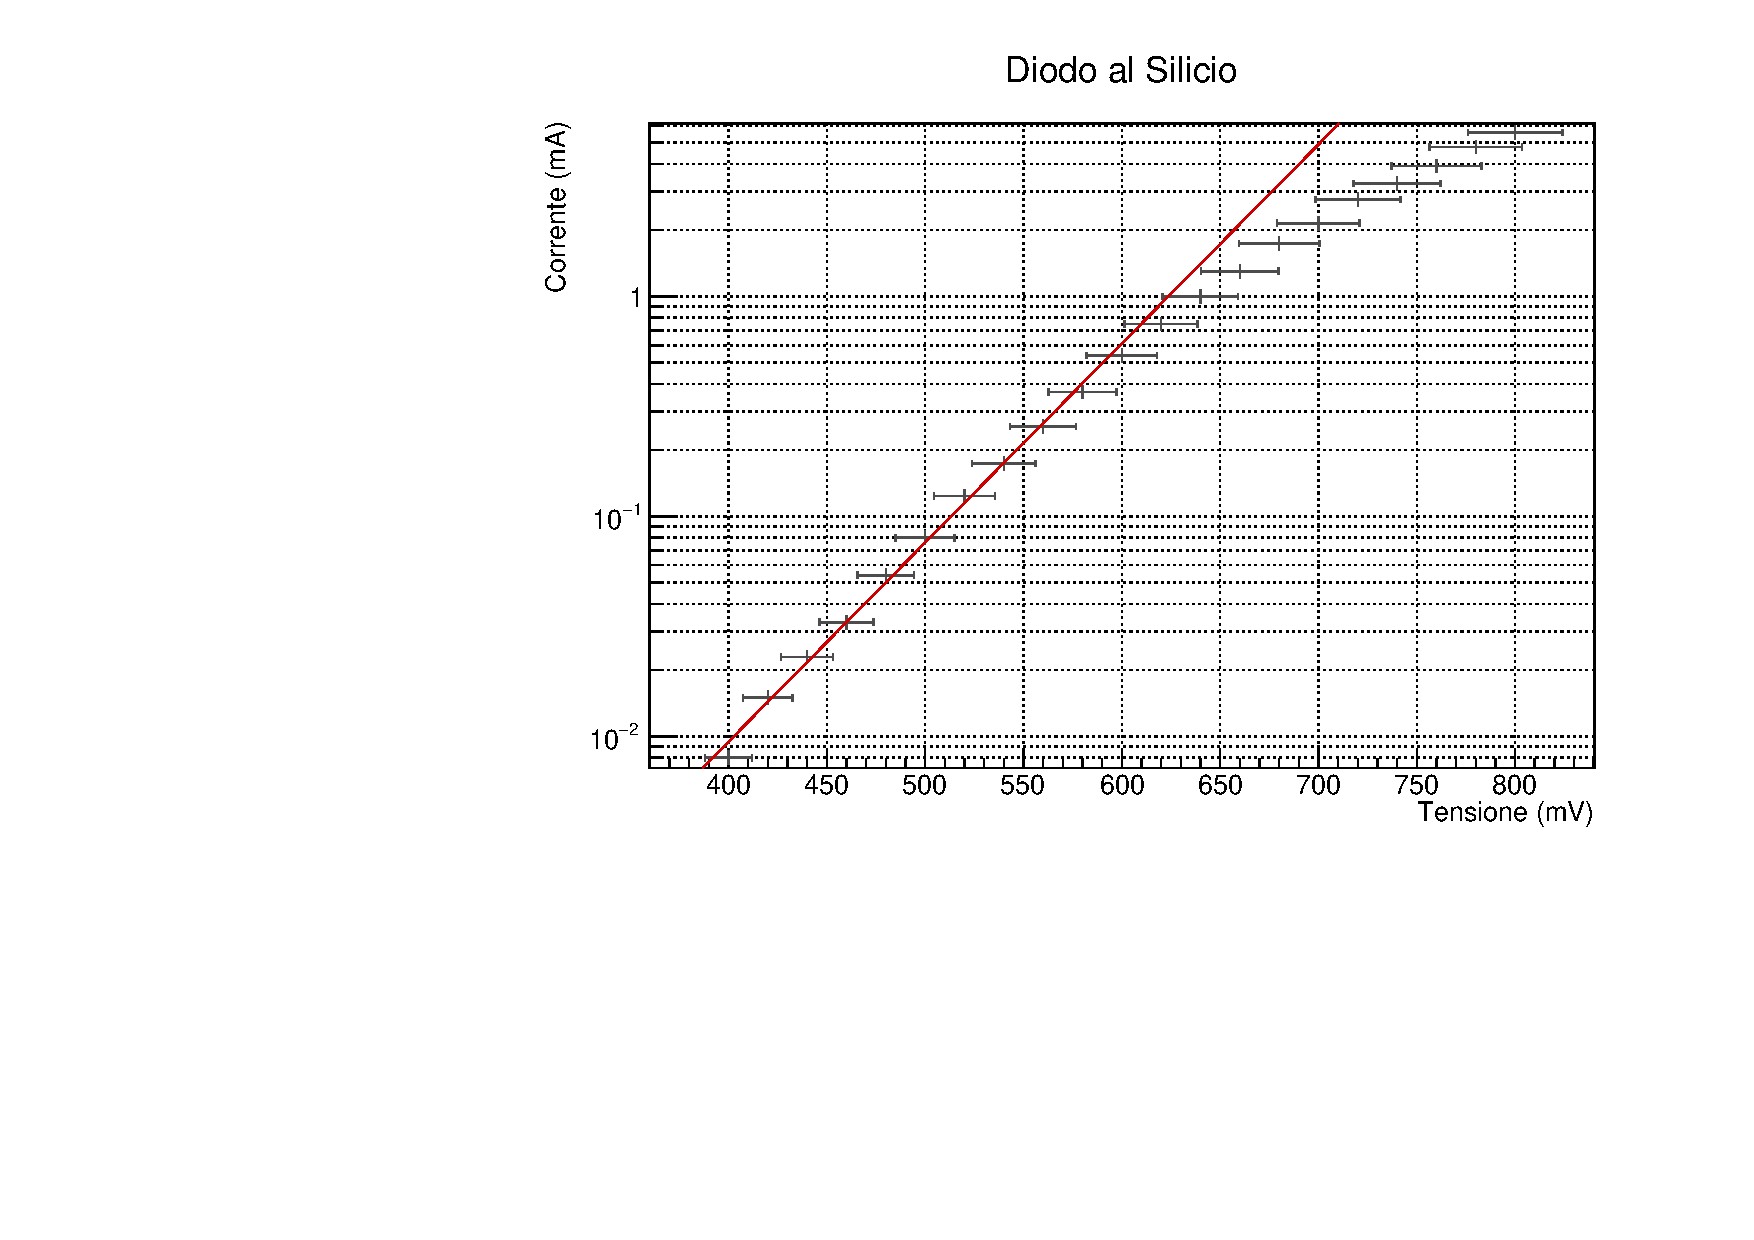
\includegraphics[width=8.25cm]{./assets/1/Silicio2.pdf}
      \caption{
        \emph{
          Caratteristica I-V del diodo al Silicio. Sono riportati i dati raccolti, assieme al fit lineare svolto sui primi punti (fino a 610mV).
        }
      }
      \label{fig:caratteristica-silicio}
    \end{subfigure}
    %
    \hspace{5mm}
    %
    \begin{subfigure}[t]{.47\textwidth}
      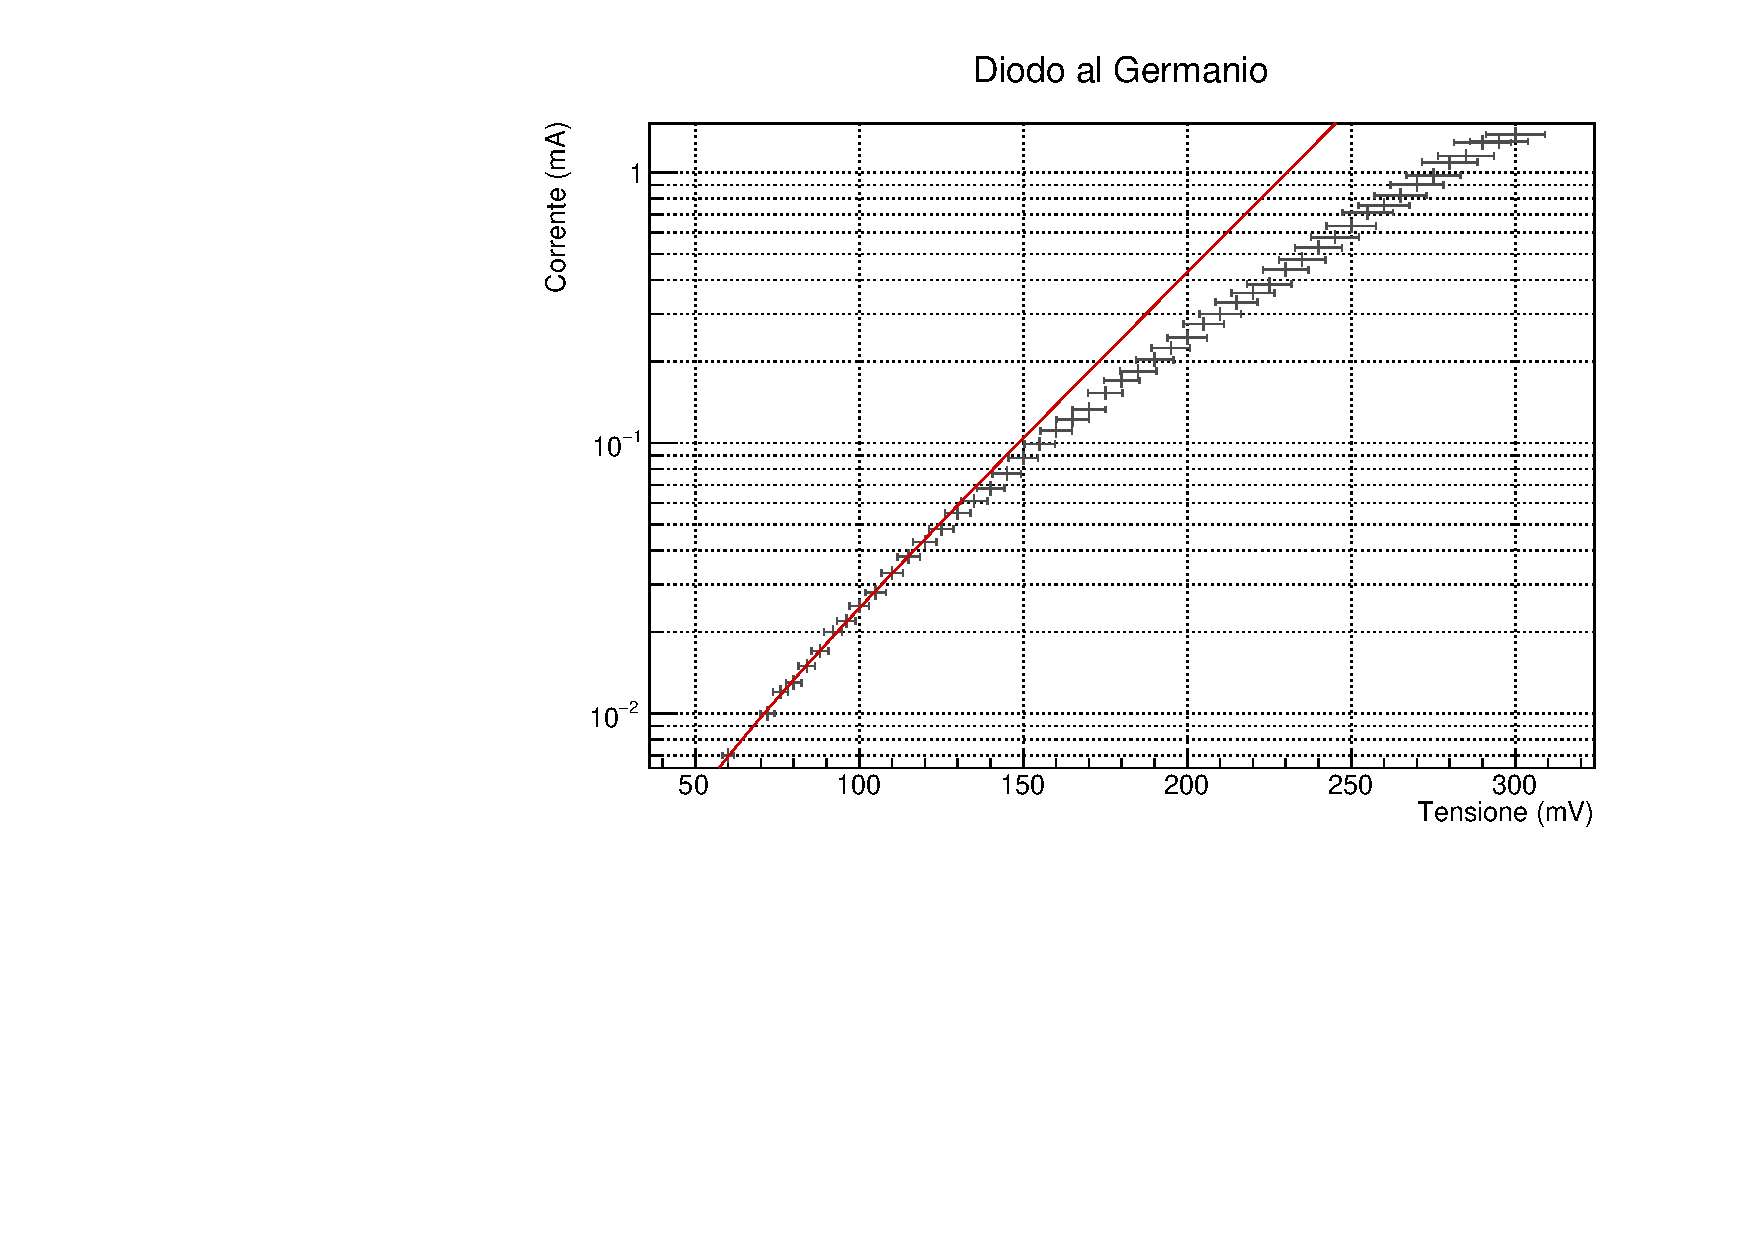
\includegraphics[width=8.25cm]{./assets/1/Germanio2.pdf}
      \caption{
        \emph{
           Caratteristica I-V del diodo al Germanio. Sono riportati i dati raccolti, assieme al fit lineare svolto sui primi punti (fino a 120mV).
        }
      }
      \label{fig:caratteristica-germanio}
    \end{subfigure}
    \caption{\emph{Dati raccolti.}
    \label{fig:caratteristiche-iv}}
  \end{figure}

\section{Conclusioni}\label{sec:conclusioni}
  Per entrambi i diodi, osserviamo qualitativamente l'andamento atteso: il plot in scala logaritmica
  è pressoché lineare fino a circa 600$mV$ per il diodo al silicio e circa 120$mV$ per il diodo al germanio.
  Quantitativamente, i valori di $\eta V_T$ sono compatibili con quelli attesi.

\newpage
\appendix
\textbf{\huge{Appendice}}
\section{Incertezze strumentali}\label{sec:incertezze-strumentali}
  \subsection{Incertezze per l'oscilloscopio}\label{subsec:incertezze-oscilloscopio}
    Nel nostro caso, l'oscilloscopio è lo strumento che introduce maggior incertezza sulle misure. Sullo schermo dello strumento,
    siamo riusciti ad apprezzare variazioni di $\frac 1 {10}$ del valore scelto come fondo scala. Per calcolare l'incertezza $\sigma$ associata
    ad una singola misura, abbiamo usato la formula \eqref{eq:incertezza-oscilloscopio}:
    \begin{equation}
      \sigma_V = \sqrt{
        \sigma_\text{casuale}^2 + \sigma_\text{sistematica}^2
      }
      \label{eq:incertezza-oscilloscopio}
    \end{equation}

    L'incertezza sistematica è fornita dal produttore dello strumento, e ha un valore di $\sigma_\text{sistematica}=3\%$.
    Per valutare l'incertezza casuale, invece, abbiamo usato la formula \eqref{eq:incertezza-oscilloscopio-casuale}:

    \begin{equation}
      \sigma_\text{casuale} = \sigma_0 + \sigma_i = 2\sigma_\text{risoluzione}
      \label{eq:incertezza-oscilloscopio-casuale}
    \end{equation}
    dove $\sigma_0$ è l'incertezza dovuta alla scelta dello zero dello strumento e
    $\sigma_i$ è l'incertezza associata alla $i$-esima misura. Abbiamo preso come valore di $\sigma_\text{risoluzione}$ la metà
    della più piccola variazione apprezzabile, ovvero: $\sigma_\text{risoluzione} = \frac 1 {20} V_\text{fondoscala}$. Si noti che le
    incertezze sullo zero e sulla misura sono considerate \emph{dipendenti}, e quindi vengono sommate linearmente.

  \subsection{Incertezze per il multimetro}\label{subsec:incertezze-multimetro}
    Le incertezze sulle misure del multimetro sono ricavate dal manuale di istruzioni del fornitore. Per il nostro multimetro,
    in tutto l'intervallo di misura, valgono $\sigma_V = \pm (0.3\% + 2\text{digit})$ e $\sigma_I = \pm (0.4\% + 2\text{digit})$, rispettivamente per le misure di tensione e corrente.

\section{Valori numerici delle misure}\label{sec:valori-misure}
  \subsection{Dati per la calibrazione}\label{subsec:valori-calibrazione}
    \begin{table}[H]
      \centering
      \begin{tabular}[t]{c|c|c||c|c|c}
        \multicolumn{3}{c}{Oscilloscopio} & \multicolumn{3}{c}{Multimetro} \\
        \toprule
        Tensione ($mV$) & Fondoscala ($mV$) & $\sigma$ ($mV$) & Tensione ($mV$) & Fondoscala ($V$) & $\sigma$ ($mV$) %
        \csvreader[
          head to column names,
        ]{./data/1/calibrazione.csv}{}% use head of csv as column names
        {\\\hline\osc&\fondoscalaOsc&\sigmaOsc&\mult&\fondoscalaMult&\sigmaMult}\\%
        \bottomrule
        \end{tabular}
      \caption{
        Dati raccolti per la calibrazione degli strumenti. Le incertezze sono riportate con una cifra significativa o
        con due cifre significative, quando la prima cifra è $1$.
      }
      \label{tab:valori-calibrazione}
    \end{table}

  \subsection{Dati relativi al silicio}\label{subsec:valori-silicio}
    \begin{table}[H]
      \centering
      \begin{tabular}[t]{c|c|c||c|c|c}
        \toprule
        $V$ ($mV$) & $V_\text{fondoscala}$ ($mV$) & $\sigma_V$ ($mV$) & $I$ ($mA$) & $I_\text{fondoscala}$ ($mA$) & $\sigma_I$ ($mA$)%
        \csvreader[
          head to column names,
        ]{./data/1/silicio.csv}{}% use head of csv as column names
        {\\\hline\V&\fondoscalaV&\sigmaV&\I&\fondoscalaI&\sigmaI}\\%
        \bottomrule
      \end{tabular}
      \caption{
        Dati raccolti relativi alla caratteristica I-V del silicio. Le incertezze sono riportate con una cifra significativa o
        con due cifre significative, quando la prima cifra è $1$.
      }
      \label{tab:valori-silicio}
    \end{table}

  \subsection{Dati relativi al germanio}\label{subsec:valori-germanio}
    \begin{table}[H]
      \centering
      \begin{tabular}[t]{c|c|c||c|c|c}
        \toprule
        $V$ ($mV$) & $V_\text{fondoscala}$ ($mV$) & $\sigma_V$ ($mV$) & $I$ ($mA$) & $I_\text{fondoscala}$ ($mA$) & $\sigma_I$ ($mA$)%
        \csvreader[
          head to column names,
        ]{./data/1/germanio.csv}{}% use head of csv as column names
        {\\\hline\V&\fondoscalaV&\sigmaV&\I&\fondoscalaI&\sigmaI}\\%
        \bottomrule
      \end{tabular}
      \caption{
        Dati raccolti relativi alla caratteristica I-V del germanio. Le incertezze sono riportate con una cifra significativa o
        con due cifre significative, quando la prima cifra è $1$.
      }
      \label{tab:valori-germanio}
    \end{table}


\bibliographystyle{unsrt} % We choose the "plain" reference style
\bibliography{./docs/reports/electronicsLabRefs.bib}

\end{document}
